Lo primero que se vio fue que, antes de llegar al acrílico, los siete rayos avanzaban paralelos y con la misma separación entre ellos, tal como salían de la máscara.

Al otro lado, todo cambió.

Los rayos salieron del cilindro inclinados hacia el centro y se juntaron muy cerca de la pieza, a una distancia bastante menor que su radio, para después cruzarse y abrirse de nuevo en forma de abanico. Así se aprecia en la figura \ref{fig:lado}, tomada desde un costado.

\begin{center}
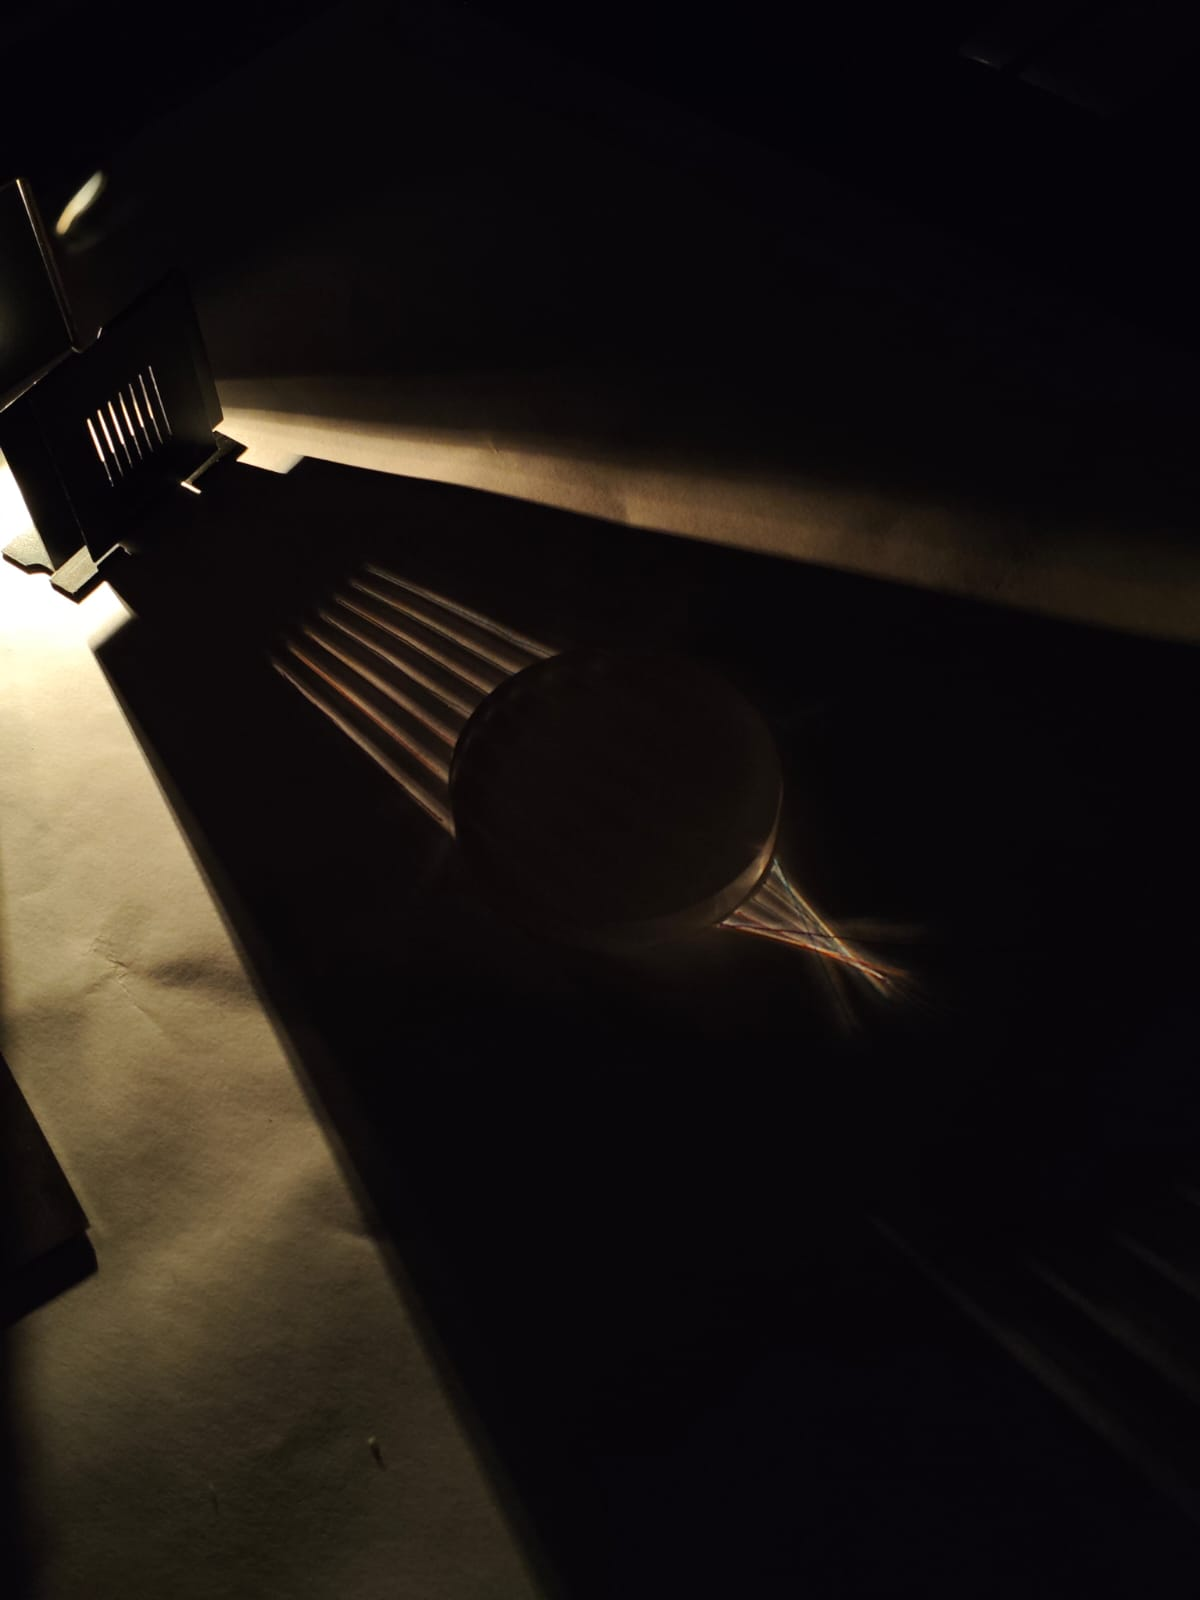
\includegraphics[width=0.8\columnwidth]{rayos_lado.jpg}
\captionof{figure}{Vista lateral. Los rayos paralelos entran por la izquierda y, al salir del cilindro, convergen y se cruzan a poca distancia de su cara de salida.}
\label{fig:lado}
\end{center}

Mirando con más atención, se notó que los rayos no se juntaban todos en un mismo punto. Los dos de las orillas se cruzaban primero, prácticamente pegados al acrílico, los siguientes un poco más adelante, y el rayo central atravesaba la pieza sin desviarse y era el último en ser alcanzado por los demás. En lugar de un punto brillante se formaba una pequeña región alargada, con forma de punta de flecha, donde las líneas se iban cruzando unas con otras.

Por último, en esa zona de cruce los rayos ya no se veían blancos. Sus bordes mostraban colores, rojizos de un lado y azulados del otro, algo que antes de entrar al acrílico no ocurría.

Para comparar con la teoría, la ecuación \eqref{eq:distancia} indica que en un cilindro de acrílico los rayos cercanos al eje deberían juntarse a $0.52\,R$ de la cara de salida. Esto coincide con lo observado: el cruce ocurrió a una distancia de aproximadamente la mitad del radio de la pieza, y no a más de tres radios, como habría pasado con una sola superficie curva según la ecuación \eqref{eq:focal}.
